Tel que trouvé dans le rapport détaillé sur le projet pilote d'entretien hivernal de la piste multifonctionnelle du pont Jacques-Cartier \parencite{pjcci_rapport_2018}, la piste multifonctionnelle du pont Jacques-Cartier (figure \ref{fig:pjcci_vueaerienne}) relie Montréal intramuros, proche de la station de métro De Lorimier / René-Lévesque, et la rive sud, à Longueuil, proche de la station de métro Longueuil et de son terminal de bus. Elle est longue d'une distance de 2.7km et est située d'un seul côté du pont, côté sud (figure \ref{fig:carte_site_etude_openstreetmap}). Elle est surtout utilisée par les cyclistes, et moindrement par les passants \parencite{pjcci_rapport_2018}.
Sa configuration est bien particulière \parencite{pjcci_fiche_2018} (figure \ref{fig:Fiche_piste-multi_pont_JC_FR_vfinale_2018-10-10}): elle ne longe pas la route adjacente sur toute sa longueur; elle est interrompue par une voie de sortie de l'ile Notre-Dame; des chicanes sont disposées à certains endroits; sa largeur varie entre 2.5m et 1.8m; elle possède une pente assez prononcée à certains moments; il y a des courbes assez serrées.
Elle est fermée l'hiver par mesure de sécurité. Elle est ouverte au début du printemps jusqu'au début de l'hiver, lorsque les conditions ne nécessitent pas d'entretien.
\begin{figure}[H]
    \centering
    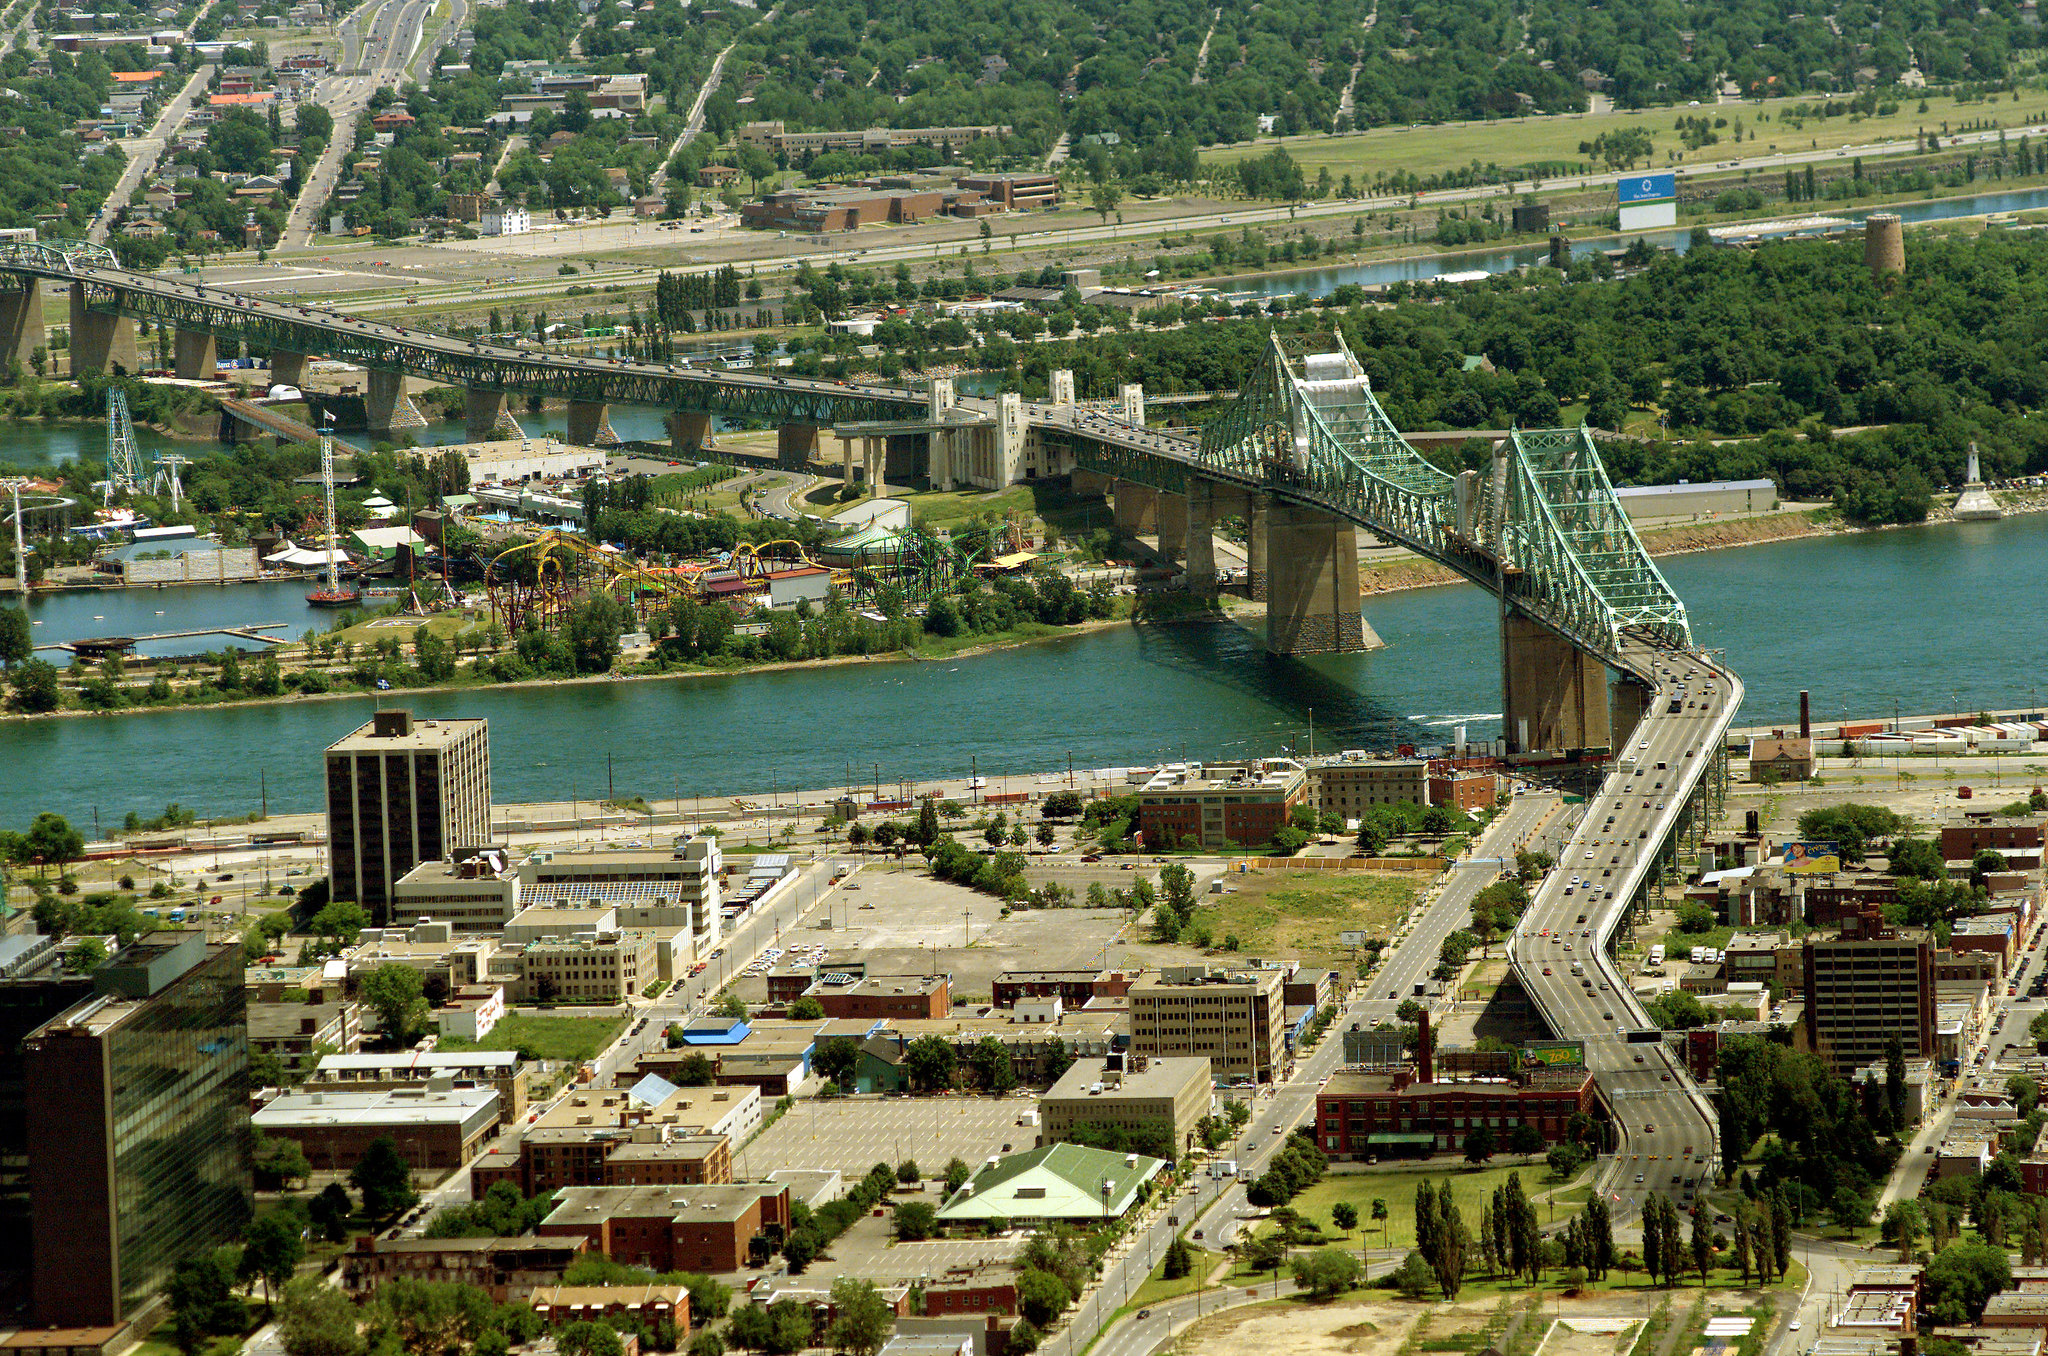
\includegraphics[width=1.0\textwidth]{pjcci_vueaerienne}
    \caption[Vue aérienne du pont Jacques-Cartier]{Vue aérienne du pont Jacques-Cartier (flickr \acrshort{pjcci})\protect\footnotemark.}
    \label{fig:pjcci_vueaerienne}
\end{figure}
\footnotetext{\url{https://www.flickr.com/photos/pjcci/6830109134}}
% \label{alamy_com_vueaerienne}
% \begin{figure}[H]
%     \centering
%     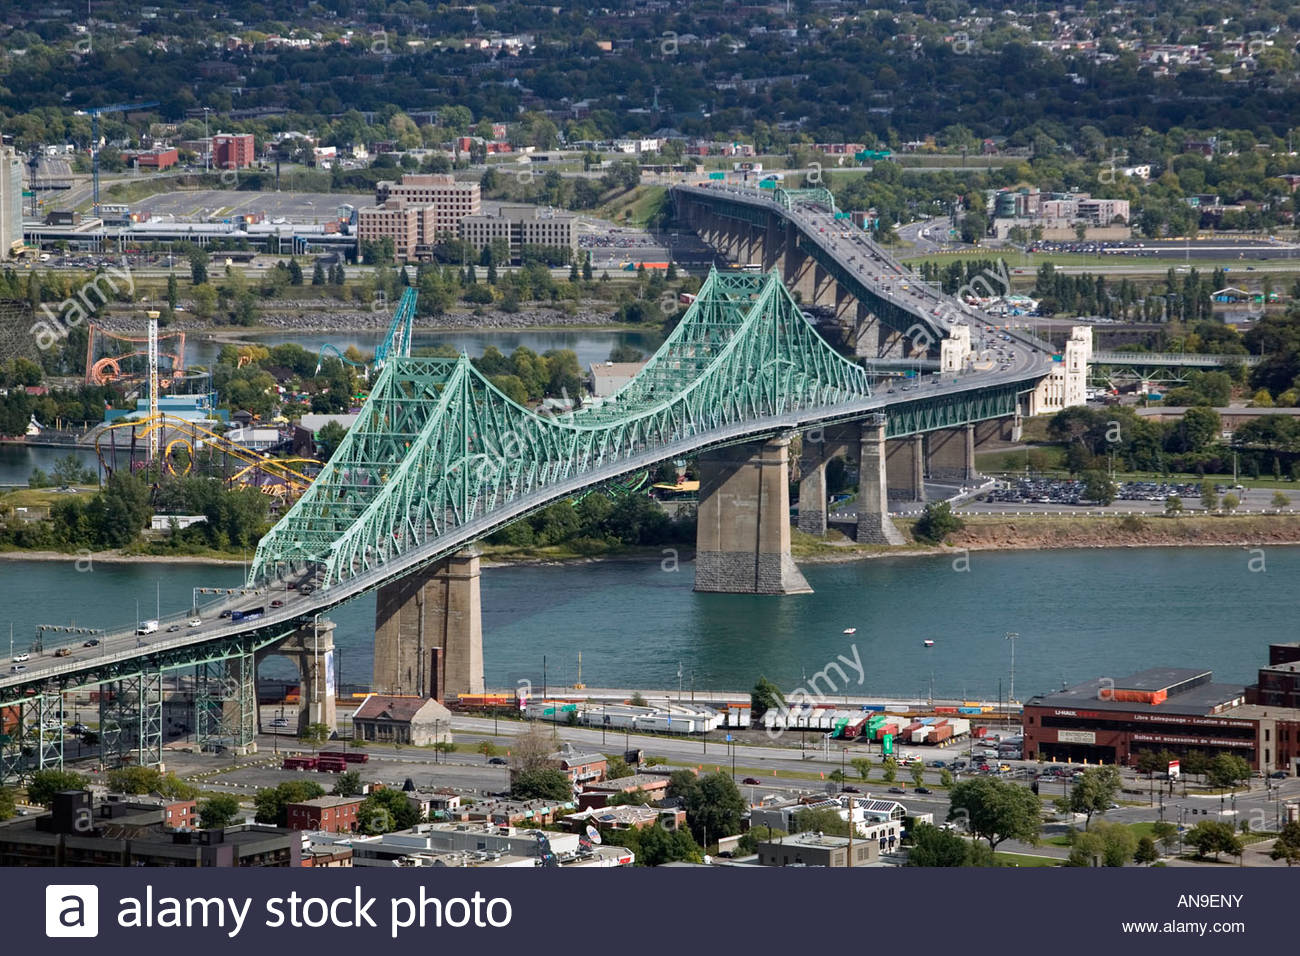
\includegraphics[width=1.0\textwidth]{alamy_com_vueaerienne}
%     \caption{Vue aérienne du pont Jacques-Cartier}
%     \label{fig:alamy_com_vueaerienne}
% \end{figure}
\begin{figure}[H]
    \centering
    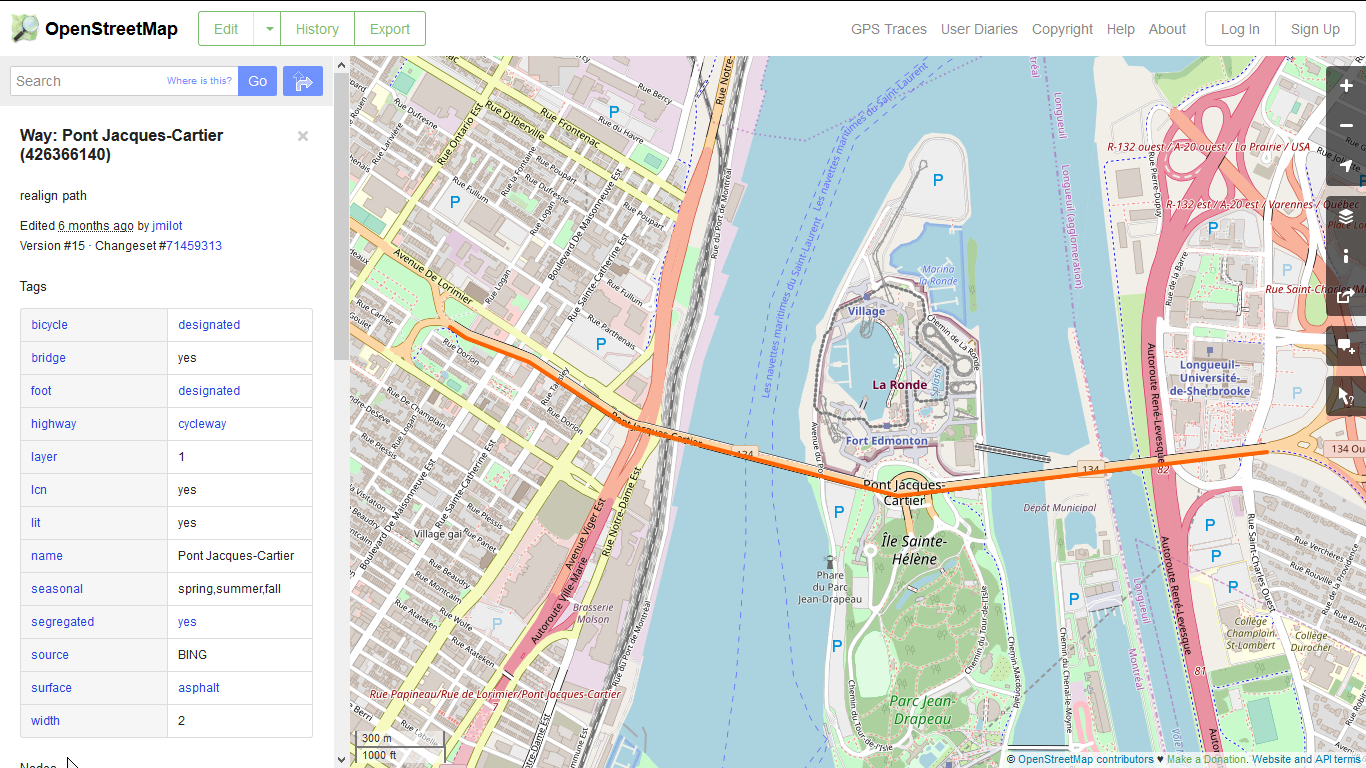
\includegraphics[width=1.0\textwidth]{carte_site_etude}
    \caption[Carte du site d'implantation]{Description de la zone géographique du site d'implantation : le pont Jacques-Cartier et la piste multifonctionnelle en orange sur le pont (copie-écran OpenStreetMap).}
    \label{fig:carte_site_etude_openstreetmap}
\end{figure}
\begin{figure}[H]
    \centering
    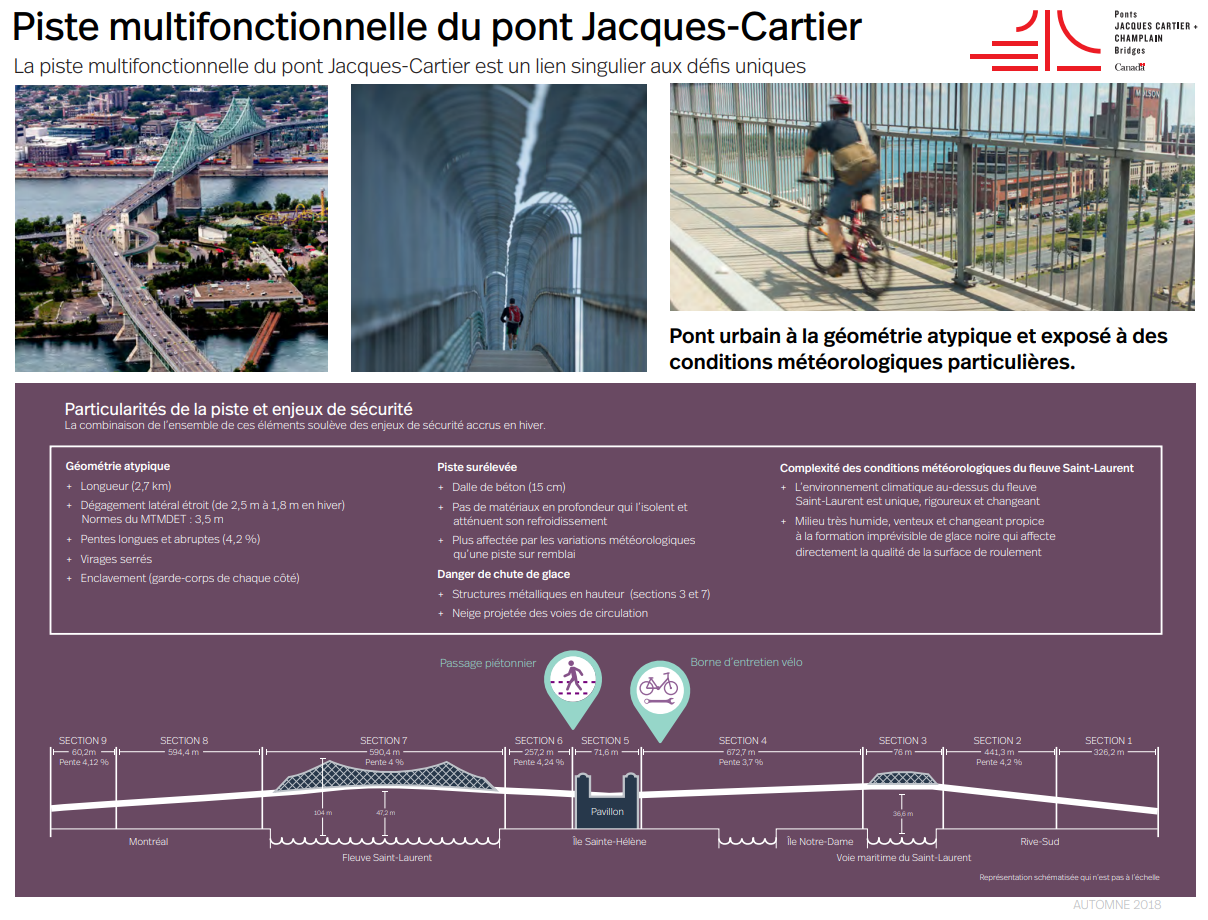
\includegraphics[width=1.0\textwidth]{Fiche_piste-multi_pont_JC_FR_vfinale_2018-10-10}
    \caption[Schéma de la configuration de la piste multifonctionnelle]{Schéma de la configuration de la piste multifonctionnelle (\acrshort{pjcci})\protect\footnotemark.}
    \label{fig:Fiche_piste-multi_pont_JC_FR_vfinale_2018-10-10}
\end{figure}
\footnotetext{\url{https://jacquescartierchamplain.ca/wp-content/uploads/2018/10/IMG_Fiche_piste-multi_pont_JC_FR_vfinale_web__2018-10-10.pdf}}